%%%%%%%%%%%%%%%%%%%%%%%%%%%%%%%%%%%%%%%%%%%%%%%%%%%%%%%%%%%%%%%%%%%%%%
% Lớp 11 | Phép biến hình phẳng | Phép đối xứng tâm
% Dạng 1C1?4-3: Xác định hình có tâm đối xứng
% Số câu: 6  (sinh tự động bởi tach_cau.py; từ nay thầy sửa trực tiếp file này)
%%%%%%%%%%%%%%%%%%%%%%%%%%%%%%%%%%%%%%%%%%%%%%%%%%%%%%%%%%%%%%%%%%%%%%

%%%%%%%%%%%%%%%% TỰ LUẬN %%%%%%%%%%%%%%%%

% nguồn: Ok_TuanLuan_Toan11_Lan1
\begin{bt}%[1C1B4-3]%[ma:0552abcb]
	Giải phương trinh: 
	\begin{listEX}[3]
		\item $\sin  \left(2x+\dfrac{\pi}{4}\right)=\sin x$;
		\item $\sin 2x=\cos 3x$; 
		\item $\cos^2 2x =\cos^2 \left(x+\dfrac{\pi}{6}\right)$. 
	\end{listEX}
	 \loigiai{
		\begin{listEX}[1]
			 \item Ta có
			 \[\sin \left(2x+\dfrac{\pi}{4}\right)=\sin x
			\Leftrightarrow 
			 \hoac{&2x+\dfrac{\pi}{4}=x+k2\pi\\&2x+\dfrac{\pi}{4}=\pi-x+k2\pi}
			\Leftrightarrow\hoac{&x=-\dfrac{\pi}{4}+k2\pi\\&3x=-\dfrac{\pi}{4}+k2\pi} \Leftrightarrow \hoac{&x=-\dfrac{\pi}{4}+k2\pi\\&x=-\dfrac{\pi}{12}+\dfrac{k2\pi}{3} 
			} (k\in  \mathbb{Z}).\]
			\item Ta  có
			\allowdisplaybreaks 
			\begin{eqnarray*}
				\sin  2x=\cos 3x &\Leftrightarrow& \cos 3x =\cos \left(\dfrac{\pi}{2}-2x\right)\\
				&\Leftrightarrow&  \hoac{
				 &3x=\dfrac{\pi}{2}-2x+k2\pi\\
				&3x=\pi-\left(\dfrac{\pi}{2}-2x\right) +k2\pi}\\ 
				&\Leftrightarrow& 
				\hoac{&5x=\dfrac{\pi}{2}+k2\pi\\&x=\dfrac{\pi}{2}+k2\pi}\\ 
				 &\Leftrightarrow&
				\hoac{&x=\dfrac{\pi}{12}+\dfrac{k2\pi}{5}\\ 
				&x=\dfrac{\pi}{2}+k2\pi}  (k\in \mathbb{Z}).
			\end{eqnarray*}
			\item Ta có $\cos^2 2x =\cos^2 \left(x+\dfrac{\pi}{6}\right) \Leftrightarrow 
			\hoac{ 
			&\cos 2x=\cos  \left(x+\dfrac{\pi}{6}\right) \quad (1)\\
			&\cos 2x=-\cos \left(x+\dfrac{\pi}{6}\right). \quad (2) 
			}$\\ 
			+)  $(1) \Leftrightarrow \hoac{
			 &2x=x+\dfrac{\pi}{6}+k2\pi\\
			&2x=-\left(x+\dfrac{\pi}{6}\right)+k2\pi 
			}  \Leftrightarrow
			\hoac{ 
			&x=\dfrac{\pi}{6}+k2\pi\\ 
			 &3x=-\dfrac{\pi}{6}+k2\pi
			 }
			\Leftrightarrow 
			 \hoac{
			&x=\dfrac{\pi}{6}+k2\pi\\ 
			 &x=-\dfrac{\pi}{18}+\dfrac{k2\pi}{3}
			 }(k\in \mathbb{Z})$.\\
			+) $(2) \Leftrightarrow 
			\cos  2x=\cos\left[\pi- \left(x+\dfrac{\pi}{6}\right) \right]
			\Leftrightarrow 
			 \hoac{
			&2x=\pi- \left(x+\dfrac{\pi}{6}\right)+k2\pi\\ 
			 &2x=-\left[\pi- \left(x+\dfrac{\pi}{6}\right)\right]+k2\pi
			 } $
			 \[\Leftrightarrow
			\hoac{ 
			 &3x=\dfrac{5\pi}{6}+k2\pi\\
			&x=-\dfrac{5\pi}{6}+k2\pi 
			} \Leftrightarrow 
			 \hoac{
			 &x=\dfrac{5\pi}{18}+\dfrac{k2\pi}{3}\\
			 &x=-\dfrac{5\pi}{6}+k2\pi
			} (k\in\mathbb{Z}).\] 
		\end{listEX}
	 }
\end{bt}

% nguồn: Ok_TuanLuan_Toan11_Lan1
\begin{bt}%[1C1B4-3]%[ma:186b5780]
	Giải phương  trình:
	\begin{listEX}[3]
		\item $\sin  \left(2x-\dfrac{\pi}{3}\right)=-\dfrac{\sqrt{3}}{2}$;
		\item $\sin \left(3x+\dfrac{\pi}{4}\right)=-\dfrac{1}{2}$; 
		\item $\cos  \left(\dfrac{x}{2}+\dfrac{\pi}{4}\right) =\dfrac{\sqrt{3}}{2}$;
		 \item $2\cos 3x+5=3$;
		\item $3\tan x=-\sqrt{3}$; 
		 \item $\cot x-3=\sqrt{3}\left(1-\cot x\right)$.
	\end{listEX}
	 \loigiai{
		\begin{listEX}[1]
			\item  Ta có
			\allowdisplaybreaks 
			\begin{eqnarray*}
				 &&\sin \left(2x-\dfrac{\pi}{3}\right)=-\dfrac{\sqrt{3}}{2}\\
				&\Leftrightarrow&  \sin \left(2x-\dfrac{\pi}{3}\right) =\sin \left(-\dfrac{\pi}{3}\right)\\
				&\Leftrightarrow&  \hoac{
				&2x-\dfrac{\pi}{3}  =-\dfrac{\pi}{3}+k2\pi\\
				&2x-\dfrac{\pi}{3} =  \pi+\dfrac{\pi}{3}+k2\pi}\\
				&\Leftrightarrow& 
				\hoac{&2x=k2\pi\\&2x=\dfrac{5\pi}{3}  +k2\pi}\\
				&\Leftrightarrow& 
				 \hoac{&x=k\pi\\&x=\dfrac{5\pi}{6}+k\pi} (k\in \mathbb{Z}).
			\end{eqnarray*}
			\item Ta  có
			\allowdisplaybreaks 
			\begin{eqnarray*}
				&&\sin \left(3x+\dfrac{\pi}{4}\right)=-\dfrac{1}{2}  \\
				&\Leftrightarrow& \sin \left(3x+\dfrac{\pi}{4}\right) =\sin  \left(-\dfrac{\pi}{6}\right)\\
				&\Leftrightarrow&  \hoac{
				 &3x+\dfrac{\pi}{4} = -\dfrac{\pi}{6}+k2\pi\\
				&3x+\dfrac{\pi}{4}=\pi -\left(-\dfrac{\pi}{6}\right)+k2\pi} \\ 
				&\Leftrightarrow& 
				\hoac{ 
				&3x=  -\dfrac{5\pi}{12}+k2\pi\\
				&3x=\dfrac{11\pi}{12}+k2\pi}  \\
				&\Leftrightarrow& 
				\hoac{&x=-\dfrac{5}{36}+\dfrac{k2\pi}{3}\\ 
				&x=\dfrac{11\pi}{36}+\dfrac{k2\pi}{3}}  (k\in \mathbb{Z}).
			\end{eqnarray*}
			\item Ta có 
			 \allowdisplaybreaks
			\begin{eqnarray*}
				&&\cos \left(\dfrac{x}{2}+\dfrac{\pi}{4}\right) =\dfrac{\sqrt{3}}{2} \\ &\Leftrightarrow&  \cos \left(\dfrac{x}{2}+\dfrac{\pi}{4}\right)=\cos \dfrac{\pi}{6}\\
				&\Leftrightarrow& \hoac{ 
				&\dfrac{x}{2}+\dfrac{\pi}{4}  = \dfrac{\pi}{6}+k2\pi\\
				&\dfrac{x}{2}+\dfrac{\pi}{4}=  -\dfrac{\pi}{6}+k2\pi}\\
				 &\Leftrightarrow&
				 \hoac{
				&\dfrac{x}{2}=-\dfrac{\pi}{12}+k2\pi\\ 
				&\dfrac{x}{2}=-\dfrac{5\pi}{12}+k2\pi}\\ 
				&\Leftrightarrow& 
				 \hoac{
				&x=-\dfrac{\pi}{6}+k4\pi\\ 
				&x=-\dfrac{5\pi}{6}+k4\pi} (k\in \mathbb{Z}). 
			\end{eqnarray*}
			\item Ta có $2\cos 3x+5=3 \Leftrightarrow \cos 3x =-1 \Leftrightarrow 3x=\pi+k2\pi \Leftrightarrow x = \dfrac{\pi}{3}+\dfrac{k2\pi}{3}\,\,(k\in  \mathbb{Z})$.
			\item Ta có $3\tan x=-\sqrt{3} \Leftrightarrow \tan x =-\dfrac{\sqrt{3}}{3}  \Leftrightarrow
			\tan x=\tan \left(-\dfrac{\pi}{6}\right) \Leftrightarrow x=-\dfrac{\pi}{6}+k\pi\,\, (k\in  \mathbb{Z}).$
			\item Ta có 
			 \allowdisplaybreaks
			\begin{eqnarray*}
				 &&\cot x-3=\sqrt{3}\left(1-\cot x\right)\\
				&\Leftrightarrow& \cot  x-3 =\sqrt{3}-\sqrt{3}\cot x\\
				&\Leftrightarrow&  (1+\sqrt{3})\cot x=\sqrt{3}(1+\sqrt{3})\\
				&\Leftrightarrow& \cot x=\sqrt{3}\\ 
				&\Leftrightarrow&  \cot x=\cot \dfrac{\pi}{6}\\
				&\Leftrightarrow&  x=\dfrac{\pi}{6}+k\pi\,\, (k\in \mathbb{Z}).
			\end{eqnarray*}
		\end{listEX}
	} 
\end{bt}

% nguồn: Ok_TuanLuan_Toan11_Lan1
\begin{bt}%[1C1B4-3]%[ma:50079815]
	Dùng đồ thị hàm  số $y=\sin x$, $y=\cos x$ để xác định số nghiệm của phương trình
	\begin{listEX}[2]
		\item  $3\sin x+2=0$ trên khoảng $\left(-\dfrac{5\pi}{2};\dfrac{5\pi}{2}\right)$;
		 \item $\cos x=0$ trên đoạn $\left[-\dfrac{5\pi}{2};\dfrac{5\pi}{2}\right]$.
	\end{listEX}
	 \loigiai{
		\begin{listEX}[1]
			\item $3\sin x+2=0$ trên  khoảng $\left(-\dfrac{5\pi}{2};\dfrac{5\pi}{2}\right)$.
			\begin{center}
				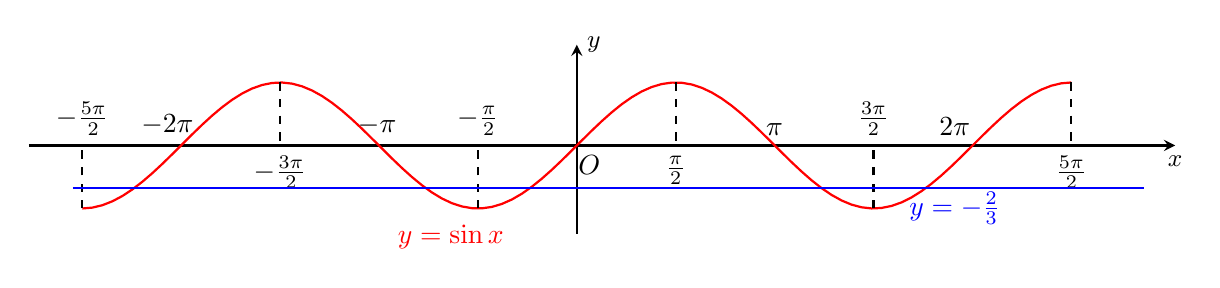
\begin{tikzpicture}[thick,>=stealth,x=1cm,y=1cm,scale=0.8]
						\draw[->] (-8.7,0) -- (9.5,0) node[below]  {\small $x$};
						\draw[->] (0,-1.4)-- (0,1.6) node[right] {\small  $y$};
						\draw[thick,red,samples=100,domain=-7.85:7.85] plot (\x,{sin  ((\x)*180/pi)});
						\draw (-3.17,0)  node[above] {$-\pi$};
						\draw  (-6.5,0) node[above] {$-2\pi$};
						\draw (3.14,0)  node[above] {$\pi$};
						\draw (6,0)  node[above] {$2\pi$};
						\draw  (0.2,0) node[below] {$O$};
						\draw[dashed] (1.57,1)--(1.57,0)  node[below] {$\frac{\pi}{2}$};
						\draw[dashed] (4.71,-1)--(4.71,0) node[above] {$\frac{3\pi}{2}$}; 
						\draw[dashed] (7.85,1)--(7.85,0) node[below] {$\frac{5\pi}{2}$}; 
						\draw[dashed] (-1.57,-1)--(-1.57,0) node[above] {$-\frac{\pi}{2}$}; 
						\draw[dashed] (-4.71,1)--(-4.71,0) node[below] {$-\frac{3\pi}{2}$}; 
						\draw[dashed] (-7.85,-1)--(-7.85,0) node[above]  {$-\frac{5\pi}{2}$};
						\draw (-2,-1.8) node[above,color=red] {$y=\sin x$}; 
						\draw[thick,blue] (-8,-0.67)--(9,-0.67); 
						 \draw (6,-1) node[color=blue] {$y=-\frac{2}{3}$};
					\end{tikzpicture}
			\end{center}
			Dựa đồ thị hàm  số $y=\sin x$ ta thấy phương trình $3\sin x+2=0$ có $5$ nghiệm trên khoảng $\left(-\dfrac{5\pi}{2};\dfrac{5\pi}{2}\right)$.
			\item  $\cos x=0$ trên đoạn $\left[-\dfrac{5\pi}{2};\dfrac{5\pi}{2}\right]$.
			\begin{center}
				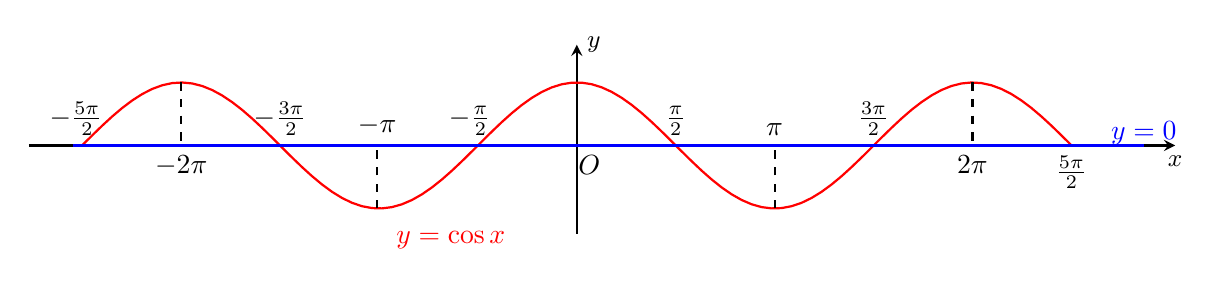
\begin{tikzpicture}[thick,>=stealth,x=1cm,y=1cm,scale=0.8]
						\draw[->] (-8.7,0)  -- (9.5,0) node[below] {\small $x$};
						\draw[->] (0,-1.4)-- (0,1.6) node[right] {\small $y$}; 
						 \draw[thick,red,samples=100,domain=-7.85:7.85] plot (\x,{cos ((\x)*180/pi)});
						\draw  [dashed] (-3.17,-1)--(-3.17,0) node[above] {$-\pi$};
						\draw [dashed] (3.14,-1)--(3.14,0) node[above] {$\pi$}; 
						\draw [dashed] (6.28,1)--(6.28,0)  node[below] {$2\pi$};
						 \draw [dashed] (-6.28,1)--(-6.28,0) node[below] {$-2\pi$};
						\draw (0.2,0) node[below] {$O$}; 
						\draw (1.57,0) node[above]  {$\frac{\pi}{2}$};
						\draw (4.71,0)  node[above] {$\frac{3\pi}{2}$};
						 \draw (7.85,0) node[below] {$\frac{5\pi}{2}$};
						\draw (-1.7,0) node[above]  {$-\frac{\pi}{2}$};
						\draw (-4.71,0)  node[above] {$-\frac{3\pi}{2}$};
						\draw  (-7.95,0) node[above] {$-\frac{5\pi}{2}$};
						 \draw (-2,-1.8) node[above,color=red] {$y=\cos x$};
						\draw[thick,blue]  (-8,0)--(9,0);
						\draw (9,0.2) node[color=blue]  {$y=0$};
					\end{tikzpicture}
			\end{center}
			Dựa vào đồ thị hàm số $y=\cos x$ ta thấy phương trình $\cos x=0$ có $6$ nghiệm trên  đoạn $\left[-\dfrac{5\pi}{2};\dfrac{5\pi}{2}\right]$.
		\end{listEX}
	} 
\end{bt}

% nguồn: Ok_TuanLuan_Toan11_Lan2
\begin{ex}%[1C1B4-3]%[ma:f660a3fc]
	 Giải phương trinh:
	\begin{listEX}[3]
		\item $\sin \left(2x+\dfrac{\pi}{4}\right)=\sin  x$;
		\item $\sin  2x=\cos 3x$;
		\item $\cos^2 2x =\cos^2 \left(x+\dfrac{\pi}{6}\right)$. 
	\end{listEX}
	 \loigiai{
		\begin{listEX}[1]
			\item Ta có 
			\[\sin \left(2x+\dfrac{\pi}{4}\right)=\sin  x
			\Leftrightarrow 
			\hoac{&2x+\dfrac{\pi}{4}=x+k2\pi\\&2x+\dfrac{\pi}{4}=\pi-x+k2\pi} 
			\Leftrightarrow\hoac{&x=-\dfrac{\pi}{4}+k2\pi\\&3x=-\dfrac{\pi}{4}+k2\pi} \Leftrightarrow \hoac{&x=-\dfrac{\pi}{4}+k2\pi\\&x=-\dfrac{\pi}{12}+\dfrac{k2\pi}{3} 
			} (k\in  \mathbb{Z}).\]
			\item  Ta có
			 \allowdisplaybreaks
			\begin{eqnarray*}
				\sin 2x=\cos 3x &\Leftrightarrow& \cos 3x =\cos  \left(\dfrac{\pi}{2}-2x\right)\\
				&\Leftrightarrow& \hoac{ 
				&3x=\dfrac{\pi}{2}-2x+k2\pi\\ 
				 &3x=\pi-\left(\dfrac{\pi}{2}-2x\right) +k2\pi}\\
				 &\Leftrightarrow&
				\hoac{&5x=\dfrac{\pi}{2}+k2\pi\\&x=\dfrac{\pi}{2}+k2\pi}\\ 
				&\Leftrightarrow& 
				\hoac{&x=\dfrac{\pi}{12}+\dfrac{k2\pi}{5}\\ 
				&x=\dfrac{\pi}{2}+k2\pi}  (k\in \mathbb{Z}).
			\end{eqnarray*}
			\item Ta có $\cos^2  2x =\cos^2 \left(x+\dfrac{\pi}{6}\right) \Leftrightarrow
			 \hoac{
			&\cos  2x=\cos \left(x+\dfrac{\pi}{6}\right) \quad (1)\\
			&\cos 2x=-\cos \left(x+\dfrac{\pi}{6}\right). \quad (2) 
			}$\\ 
			 +) $(1) \Leftrightarrow \hoac{
			 &2x=x+\dfrac{\pi}{6}+k2\pi\\
			 &2x=-\left(x+\dfrac{\pi}{6}\right)+k2\pi
			} \Leftrightarrow 
			\hoac{ 
			&x=\dfrac{\pi}{6}+k2\pi\\ 
			 &3x=-\dfrac{\pi}{6}+k2\pi
			} 
			 \Leftrightarrow
			\hoac{ 
			 &x=\dfrac{\pi}{6}+k2\pi\\
			 &x=-\dfrac{\pi}{18}+\dfrac{k2\pi}{3}
			 }(k\in \mathbb{Z})$.\\
			+) $(2)  \Leftrightarrow
			\cos  2x=\cos\left[\pi- \left(x+\dfrac{\pi}{6}\right) \right]
			 \Leftrightarrow
			 \hoac{
			&2x=\pi-  \left(x+\dfrac{\pi}{6}\right)+k2\pi\\
			&2x=-\left[\pi-  \left(x+\dfrac{\pi}{6}\right)\right]+k2\pi
			} $ 
			 \[\Leftrightarrow
			\hoac{ 
			 &3x=\dfrac{5\pi}{6}+k2\pi\\
			&x=-\dfrac{5\pi}{6}+k2\pi 
			} \Leftrightarrow 
			 \hoac{
			&x=\dfrac{5\pi}{18}+\dfrac{k2\pi}{3}\\ 
			 &x=-\dfrac{5\pi}{6}+k2\pi
			 } (k\in\mathbb{Z}).\]
		\end{listEX}
	 }
\end{ex}

% nguồn: Ok_TuanLuan_Toan11_Lan2
\begin{ex}%[1C1B4-3]%[ma:cca3d4b3]
	Giải  phương trình:
	\begin{listEX}[3]
		\item  $\sin \left(2x-\dfrac{\pi}{3}\right)=-\dfrac{\sqrt{3}}{2}$;
		\item $\sin \left(3x+\dfrac{\pi}{4}\right)=-\dfrac{1}{2}$; 
		\item  $\cos \left(\dfrac{x}{2}+\dfrac{\pi}{4}\right) =\dfrac{\sqrt{3}}{2}$;
		\item  $2\cos 3x+5=3$;
		\item  $3\tan x=-\sqrt{3}$;
		\item $\cot x-3=\sqrt{3}\left(1-\cot  x\right)$.
	\end{listEX}
	\loigiai{ 
		\begin{listEX}[1]
			 \item Ta có
			 \allowdisplaybreaks
			\begin{eqnarray*}
				&&\sin  \left(2x-\dfrac{\pi}{3}\right)=-\dfrac{\sqrt{3}}{2}\\
				&\Leftrightarrow& \sin  \left(2x-\dfrac{\pi}{3}\right) =\sin \left(-\dfrac{\pi}{3}\right)\\
				&\Leftrightarrow& \hoac{ 
				 &2x-\dfrac{\pi}{3} =-\dfrac{\pi}{3}+k2\pi\\
				&2x-\dfrac{\pi}{3} = \pi+\dfrac{\pi}{3}+k2\pi}\\ 
				&\Leftrightarrow& 
				\hoac{&2x=k2\pi\\&2x=\dfrac{5\pi}{3}  +k2\pi}\\
				 &\Leftrightarrow&
				 \hoac{&x=k\pi\\&x=\dfrac{5\pi}{6}+k\pi} (k\in \mathbb{Z}).
			\end{eqnarray*}
			 \item Ta có
			 \allowdisplaybreaks
			\begin{eqnarray*}
				 &&\sin \left(3x+\dfrac{\pi}{4}\right)=-\dfrac{1}{2} \\
				&\Leftrightarrow& \sin \left(3x+\dfrac{\pi}{4}\right) =\sin \left(-\dfrac{\pi}{6}\right)\\ 
				&\Leftrightarrow& \hoac{ 
				&3x+\dfrac{\pi}{4} =  -\dfrac{\pi}{6}+k2\pi\\
				&3x+\dfrac{\pi}{4}=\pi -\left(-\dfrac{\pi}{6}\right)+k2\pi}  \\
				 &\Leftrightarrow&
				\hoac{ 
				 &3x= -\dfrac{5\pi}{12}+k2\pi\\
				&3x=\dfrac{11\pi}{12}+k2\pi} \\ 
				&\Leftrightarrow& 
				 \hoac{&x=-\dfrac{5}{36}+\dfrac{k2\pi}{3}\\
				&x=\dfrac{11\pi}{36}+\dfrac{k2\pi}{3}} (k\in \mathbb{Z}). 
			\end{eqnarray*}
			 \item Ta có
			\allowdisplaybreaks 
			\begin{eqnarray*}
				&&\cos \left(\dfrac{x}{2}+\dfrac{\pi}{4}\right) =\dfrac{\sqrt{3}}{2} \\ &\Leftrightarrow& \cos \left(\dfrac{x}{2}+\dfrac{\pi}{4}\right)=\cos \dfrac{\pi}{6}\\ 
				 &\Leftrightarrow& \hoac{
				&\dfrac{x}{2}+\dfrac{\pi}{4} =  \dfrac{\pi}{6}+k2\pi\\
				&\dfrac{x}{2}+\dfrac{\pi}{4}=  -\dfrac{\pi}{6}+k2\pi}\\
				&\Leftrightarrow& 
				 \hoac{
				&\dfrac{x}{2}=-\dfrac{\pi}{12}+k2\pi\\ 
				 &\dfrac{x}{2}=-\dfrac{5\pi}{12}+k2\pi}\\
				&\Leftrightarrow& 
				\hoac{ 
				 &x=-\dfrac{\pi}{6}+k4\pi\\
				&x=-\dfrac{5\pi}{6}+k4\pi} (k\in \mathbb{Z}). 
			\end{eqnarray*}
			\item Ta có $2\cos 3x+5=3 \Leftrightarrow \cos 3x =-1 \Leftrightarrow 3x=\pi+k2\pi \Leftrightarrow x  = \dfrac{\pi}{3}+\dfrac{k2\pi}{3}\,\,(k\in \mathbb{Z})$.
			\item Ta có $3\tan x=-\sqrt{3} \Leftrightarrow \tan x =-\dfrac{\sqrt{3}}{3} \Leftrightarrow 
			\tan x=\tan \left(-\dfrac{\pi}{6}\right) \Leftrightarrow x=-\dfrac{\pi}{6}+k\pi\,\,  (k\in \mathbb{Z}).$
			\item Ta có 
			\allowdisplaybreaks 
			\begin{eqnarray*}
				&&\cot x-3=\sqrt{3}\left(1-\cot x\right)\\ 
				&\Leftrightarrow& \cot x-3 =\sqrt{3}-\sqrt{3}\cot  x\\
				 &\Leftrightarrow& (1+\sqrt{3})\cot x=\sqrt{3}(1+\sqrt{3})\\
				&\Leftrightarrow& \cot  x=\sqrt{3}\\
				&\Leftrightarrow& \cot  x=\cot \dfrac{\pi}{6}\\
				&\Leftrightarrow& x=\dfrac{\pi}{6}+k\pi\,\, (k\in  \mathbb{Z}).
			\end{eqnarray*}
		\end{listEX}
	} 
\end{ex}

% nguồn: Ok_TuanLuan_Toan11_Lan2
\begin{ex}%[1C1B4-3]%[ma:ed8f7e2e]
	 Dùng đồ thị hàm số $y=\sin x$, $y=\cos x$ để xác định số nghiệm của phương trình
	\begin{listEX}[2]
		 \item $3\sin x+2=0$ trên khoảng $\left(-\dfrac{5\pi}{2};\dfrac{5\pi}{2}\right)$;
		\item $\cos x=0$ trên đoạn  $\left[-\dfrac{5\pi}{2};\dfrac{5\pi}{2}\right]$.
	\end{listEX}
	\loigiai{ 
		\begin{listEX}[1]
			 \item $3\sin x+2=0$ trên khoảng $\left(-\dfrac{5\pi}{2};\dfrac{5\pi}{2}\right)$.
			\begin{center}
				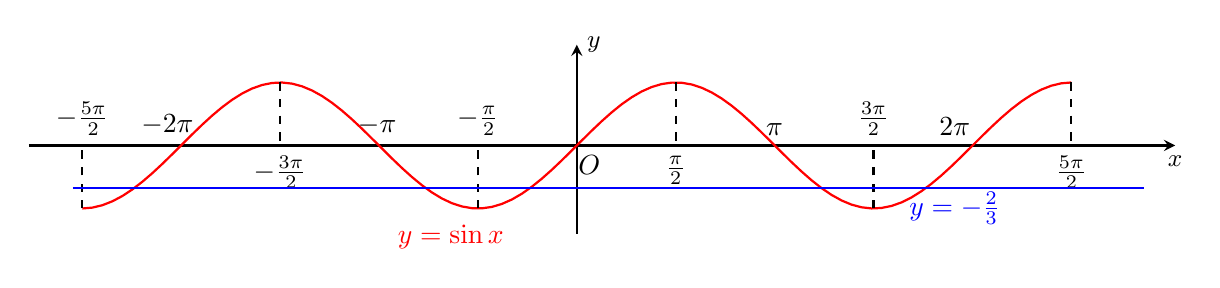
\begin{tikzpicture}[thick,>=stealth,x=1cm,y=1cm,scale=0.8]
						\draw[->] (-8.7,0) --  (9.5,0) node[below] {\small $x$};
						\draw[->]  (0,-1.4)-- (0,1.6) node[right] {\small $y$};
						\draw[thick,red,samples=100,domain=-7.85:7.85] plot  (\x,{sin ((\x)*180/pi)});
						 \draw (-3.17,0) node[above] {$-\pi$};
						\draw (-6.5,0)  node[above] {$-2\pi$};
						\draw (3.14,0) node[above] {$\pi$}; 
						\draw (6,0) node[above] {$2\pi$}; 
						\draw (0.2,0) node[below] {$O$}; 
						\draw[dashed] (1.57,1)--(1.57,0) node[below]  {$\frac{\pi}{2}$};
						 \draw[dashed] (4.71,-1)--(4.71,0) node[above] {$\frac{3\pi}{2}$};
						\draw[dashed] (7.85,1)--(7.85,0)  node[below] {$\frac{5\pi}{2}$};
						\draw[dashed] (-1.57,-1)--(-1.57,0) node[above] {$-\frac{\pi}{2}$}; 
						\draw[dashed] (-4.71,1)--(-4.71,0)  node[below] {$-\frac{3\pi}{2}$};
						\draw[dashed] (-7.85,-1)--(-7.85,0) node[above]  {$-\frac{5\pi}{2}$};
						\draw (-2,-1.8) node[above,color=red]  {$y=\sin x$};
						 \draw[thick,blue] (-8,-0.67)--(9,-0.67);
						\draw (6,-1)  node[color=blue] {$y=-\frac{2}{3}$};
					\end{tikzpicture}
			\end{center}
			Dựa  đồ thị hàm số $y=\sin x$ ta thấy phương trình $3\sin x+2=0$ có $5$ nghiệm trên khoảng $\left(-\dfrac{5\pi}{2};\dfrac{5\pi}{2}\right)$.
			\item  $\cos x=0$ trên đoạn $\left[-\dfrac{5\pi}{2};\dfrac{5\pi}{2}\right]$.
			\begin{center}
				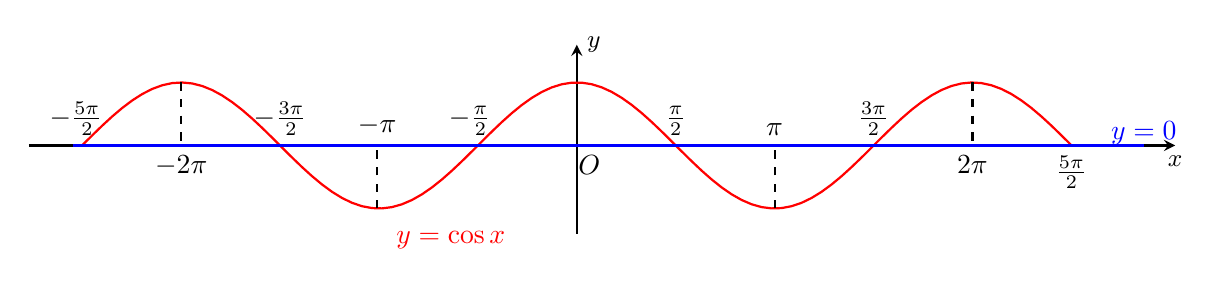
\begin{tikzpicture}[thick,>=stealth,x=1cm,y=1cm,scale=0.8]
						\draw[->] (-8.7,0) --  (9.5,0) node[below] {\small $x$};
						\draw[->] (0,-1.4)-- (0,1.6)  node[right] {\small $y$};
						\draw[thick,red,samples=100,domain=-7.85:7.85] plot  (\x,{cos ((\x)*180/pi)});
						\draw [dashed] (-3.17,-1)--(-3.17,0)  node[above] {$-\pi$};
						\draw [dashed] (3.14,-1)--(3.14,0)  node[above] {$\pi$};
						\draw [dashed] (6.28,1)--(6.28,0)  node[below] {$2\pi$};
						 \draw [dashed] (-6.28,1)--(-6.28,0) node[below] {$-2\pi$};
						\draw (0.2,0) node[below] {$O$}; 
						\draw (1.57,0) node[above]  {$\frac{\pi}{2}$};
						\draw  (4.71,0) node[above] {$\frac{3\pi}{2}$};
						 \draw (7.85,0) node[below] {$\frac{5\pi}{2}$};
						 \draw (-1.7,0) node[above] {$-\frac{\pi}{2}$};
						\draw  (-4.71,0) node[above] {$-\frac{3\pi}{2}$};
						 \draw (-7.95,0) node[above] {$-\frac{5\pi}{2}$};
						\draw (-2,-1.8) node[above,color=red] {$y=\cos x$}; 
						\draw[thick,blue] (-8,0)--(9,0); 
						\draw (9,0.2) node[color=blue] {$y=0$}; 
					\end{tikzpicture}
			\end{center}
			Dựa vào đồ thị hàm số $y=\cos x$ ta thấy phương trình $\cos x=0$ có $6$ nghiệm trên đoạn  $\left[-\dfrac{5\pi}{2};\dfrac{5\pi}{2}\right]$.
		\end{listEX}
	 }
\end{ex}
